\section{Flowchart}
A flowchart is a type of diagram that represents an algorithm, work flow or process, showing the steps as boxes of various kinds, and their order by connecting them with arrows
and the flowchart \ref{fig:FD1} of Democratic maps showing the flow of control and Data in the software.

\begin{figure}
	\centering 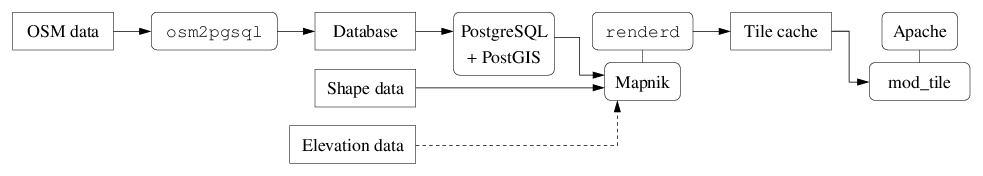
\includegraphics[width=\linewidth]{input/images/osmserv.png}
	\caption{Flowchart of Democratic Maps}
	\label{fig:FD1}
\end{figure}

\subsection{Detailed Description}

The basic implementation of this project is almost done in form of prototype. There is need to modify the structure of the project. We have to divide the task into there parts:

\begin{enumerate}
	\item \textbf{Front end}
	It will deal with how the Democratic maps will look to the user like in form of toolbars, menus etc. This part will include two parts:
	\begin{enumerate}
		\item \textbf{Rebar Addon toolbar/menus}
		It contains a list of different animations.
		\item \textbf{Dialog box}
		User can input latitude and longitude of the point to locate the point.
	\end{enumerate}

\begin{figure}[h!]
	\centering
	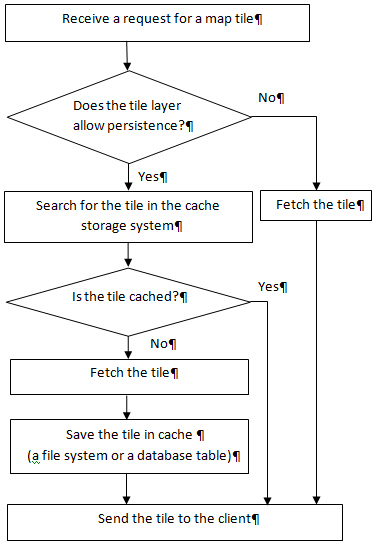
\includegraphics[scale=0.9]{input/images/fetch.jpg}
	\caption{Flow Chart to Serve a Tile}
\end{figure}
\hspace{-1.7em}

	
	\item \textbf{Back End}
       The slippymap send to render the tiles on the fly. The tiles are stored for caching the tiles mapnik creates the tiles. The utility osm2pgsql is used to convert raw data to postgresql database. At backend openstreetma-carto fetch the database and create beautiful maps and displayed on the browser. 	
\end{enumerate}

\subsection{DFD's}
A data flow diagram (DFD) is a graphical representation of the "flow" of data through an information system, modeling its process aspects. A DFD is often used as a preliminary step to create an overview of the system, which can later be elaborated. DFDs to serve a tile is as following-:
\begin{figure}[h!]
	\centering
	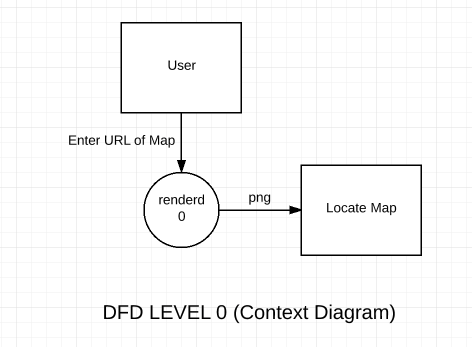
\includegraphics[scale=0.6]{input/images/DFD_0.png}
	\caption{Data Flow Diagram Level 0}
\end{figure}
\begin{figure}[h!]
	        \centering
		        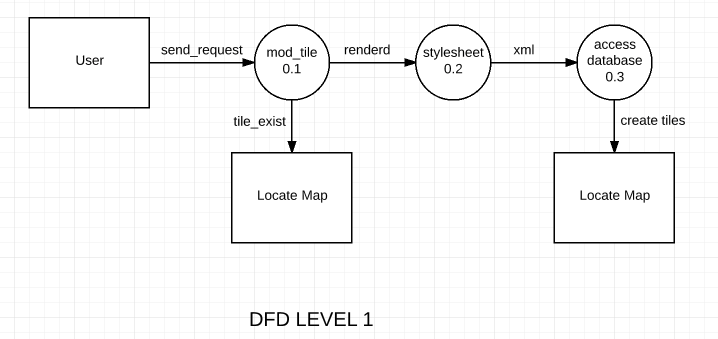
\includegraphics[scale=0.6]{input/images/DFD_1.png}
			        \caption{Data Flow Diagram Level 1}
\end{figure}
\begin{figure}[h!]
	        \centering
		        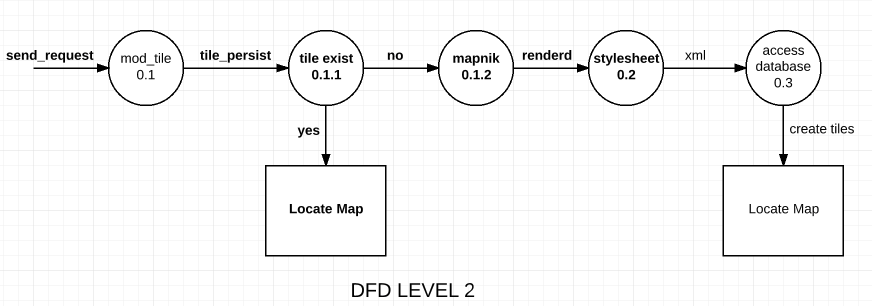
\includegraphics[scale=0.6]{input/images/DFD_2.png}
			        \caption{Data Flow Diagram Level 2}
\end{figure}

